\documentclass{beamer}

\usepackage[version=4]{mhchem}  
\usepackage{tikz}
\usepackage[
    backend=biber,
    style=numeric,
    sorting=ynt
]{biblatex}

% \bibliography{bibliografija}

\usetheme{Copenhagen}

%Information to be included in the title page:
\title{Sample title}
\author{Anonymous}
\institute{Overleaf}
\date{2025}

\title[]
{Medžiagų maišymo modeliavimas cheminėse reakcijose}

\subtitle{Modelling the mixing of reagents in chemical reactions}

\author[Arnas Vaicekauskas]
{
    A.~Vaicekauskas\inst{1}\\ 
    \small Darbo vadovas: Asist. Dr. R.~Astrauskas\inst{1}
}

\institute[MIF]
{
  \inst{1}
  Matematikos ir informatikos fakultetas\\
  Vilniaus Universitetas
}


\begin{document}

\frame{\titlepage}

\begin{frame}
\frametitle{Ytrio aliuminio granatas (YAG)}

\begin{figure}
    \centering
    \begin{minipage}{.5\textwidth}
        \centering
        \includegraphics[width=0.8\textwidth]{slides/assets/nd:yag.png}
    \end{minipage}%
    \begin{minipage}{.5\textwidth}
               
    \end{minipage}
\end{figure}

\begin{itemize}
    \item Plačiausiai naudojama medžiaga lazerių aktyviosioms terpėms gaminti
    \item YAG lazeriai naudojami medicinos bei gamybos srityse
\end{itemize}

\end{frame}

\begin{frame}
\frametitle{YAG cheminė reakcija}

\centering
\begin{align*}
    \ce{3Y_2O_3 + 5Al_2O_3 -> 2Y_3Al_5O_{12}}
\end{align*}    
\begin{itemize}
\item YAG kristalai sintezuojami kaitinant Aliuminio ir Itrio oksidų mišinį
\item Reakcija gali užtrukti keliolika valandų
\item Chemikai vykstant reakcijai periodiškai išmaišo reagentus, kad reakcijos laikas sutrumpėtų
\end{itemize}

\end{frame}

\begin{frame}
\frametitle{Darbo apimtis}
\textbf{Tikslas} - sukurti kompiuterinį YAG reakcijos maišymo modelį ir jį ištirti.

\textbf{Uždaviniai:}
\begin{enumerate}
\item Sukurti kompiuterinį YAG reakcijos modelį
\item Patikrinti kompiuterinio modelio rezultatų korektiškumą
\item Papildyti kompiuterinį modelį su maišymo procesu
\item Ištirti kompiuterinio modelio rezultatus
\end{enumerate}

\end{frame}

\begin{frame}
\frametitle{Matematinis modelis}

\begin{align*}
    \frac{\partial c_1}{\partial t} & =-3kc_1c_2+D\left(\frac{\partial^2c_1}{\partial x^2}+\frac{\partial^2c_1}{\partial y^2}\right) \\
    \frac{\partial c_2}{\partial t} & =-5kc_1c_2+D\left(\frac{\partial^2c_2}{\partial x^2}+\frac{\partial^2c_2}{\partial y^2}\right)\\
    \frac{\partial c_3}{\partial t} & =2kc_1c_2
\end{align*}

\end{frame}

\begin{frame}
    \frametitle{Pradinės ir kraštinės sąlygos}
    \begin{figure}
        \centering
        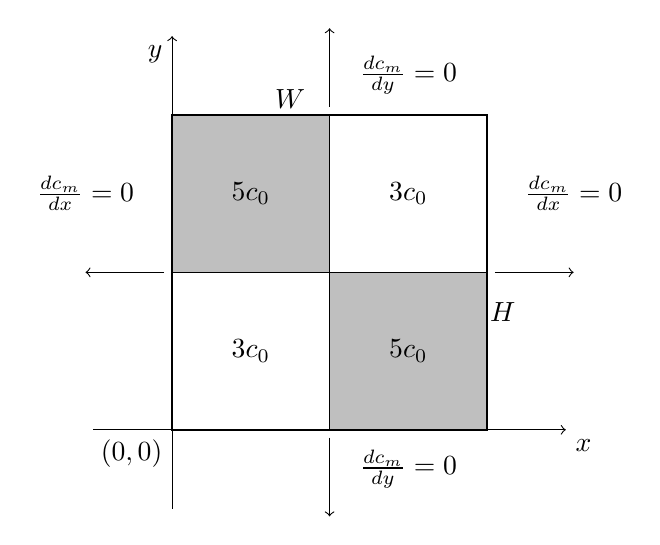
\begin{tikzpicture}[scale=2.0]
            \draw[fill=white] (0,0) rectangle (1,1);
            \draw[fill=white] (1,1) rectangle (2,2);
            \draw[fill=gray!50] (0,1) rectangle (1,2);
            \draw[fill=gray!50] (1,0) rectangle (2,1);
    
            % Draw the boundary of the square
            \draw[thick] (0,0) rectangle (2,2);
    
            % Draw axes
            \draw[->] (-0.5, 0) -- (2.5, 0) node[anchor=north west] {$x$};
            \draw[->] (0, -0.5) -- (0, 2.5) node[anchor=north east] {$y$};
    
            % Mark the origin
            \node[anchor=north east] at (0,0) {$(0, 0)$};
    
            % Mark the side length
            \draw[-] (2,0) -- (2,2);
            \draw[-] (0,2) -- (2,2);

            \node at (2.1, 0.75) {$H$};
            \node at (0.75, 2.1) {$W$};
            
            \draw (0.5, 1.5) node[anchor=center] {$5c_0$};
            \draw (1.5, 0.5) node[anchor=center] {$5c_0$};
            \draw (1.5, 1.5) node[anchor=center] {$3c_0$};
            \draw (0.5, 0.5) node[anchor=center] {$3c_0$};

            % boundary conditions
            \draw[->] (-0.05,1) -- (-0.55,1);
            \node at (-0.55, 1.5) {$\frac{dc_m}{dx} = 0$};

            \draw[->] (2.05,1) -- (2.55,1);
            \node at (2.55, 1.5) {$\frac{dc_m}{dx} = 0$};

            \draw[->] (1, -0.05) -- (1, -0.55);
            \node at (1.5, -0.25) {$\frac{dc_m}{dy} = 0$};

            \draw[->] (1, 2.05) -- (1, 2.55);
            \node at (1.5, 2.25) {$\frac{dc_m}{dy} = 0$};

        \end{tikzpicture}
    \end{figure}
\end{frame}

\begin{frame}
    \frametitle{Stabilumas}
    \begin{align*}
        \Delta t \leqslant \left(15kc_0+2D\left((\Delta x)^{-2}+(\Delta y)^{-2}\right)\right)^{-1}
    \end{align*}
\end{frame}

\begin{frame}
    \frametitle{Reakcijos modelio rezultatai}
    \centering
    \includegraphics[width=12cm]{paper/assets/example-0.png} \\ 
    \includegraphics[width=12cm]{paper/assets/example-2.png}

\end{frame}

\begin{frame}
\frametitle{Atsitiktinis maišymas}
\centering
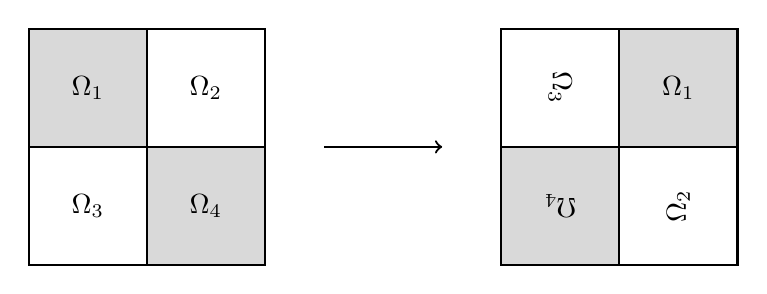
\begin{tikzpicture}[scale=1.5]

    \fill[gray!30] (0,1) rectangle (1, 2);
    \fill[gray!30] (1,0) rectangle (2, 1);

    % Original Grid
    \draw[thick] (0,0) rectangle (2,2);
    \draw[thick] (1,0) -- (1,2);
    \draw[thick] (0,1) -- (2,1);

    \node at (0.5,1.5) {$\Omega_1$};
    \node at (1.5,1.5) {$\Omega_2$};
    \node at (0.5,0.5) {$\Omega_3$};
    \node at (1.5,0.5) {$\Omega_4$};

    % Arrow
    \draw[->, thick] (2.5,1) -- (3.5,1);

    % Transformed Grid
    \begin{scope}[shift={(4,0)}]

        \fill[gray!30] (0,0) rectangle (1, 1);
        \fill[gray!30] (1,1) rectangle (2, 2);

        \draw[thick] (0,0) rectangle (2,2);
        \draw[thick] (1,0) -- (1,2);
        \draw[thick] (0,1) -- (2,1);

        \node at (0.5,1.5) {\rotatebox{270}{$\Omega_3$}}; % Rotated 180° horizontally
        \node at (1.5,1.5) {$\Omega_1$};             % No change
        \node at (0.5,0.5) {\rotatebox{180}{$\Omega_4$}}; % Upside down
        \node at (1.5,0.5) {\rotatebox{90}{$\Omega_2$}};  % 90° rotation
    \end{scope}
\end{tikzpicture}
\end{frame}

\begin{frame}
    \frametitle{Atsitiktinio maišymo rezultatai}
    \centering
    \includegraphics[width=12cm]{paper/assets/random-mix-example-c0-1.png} \\
    \includegraphics[width=12cm]{paper/assets/random-mix-example-c2-1.png}
\end{frame}

\begin{frame}
    \frametitle{Atsitiktinio maišymo rezultatai}
    \centering
    \includegraphics[width=10cm]{paper/assets/bad-mix-qnt-compare-1.png}
\end{frame}

\begin{frame}
\frametitle{Tobulas maišymas}
\centering
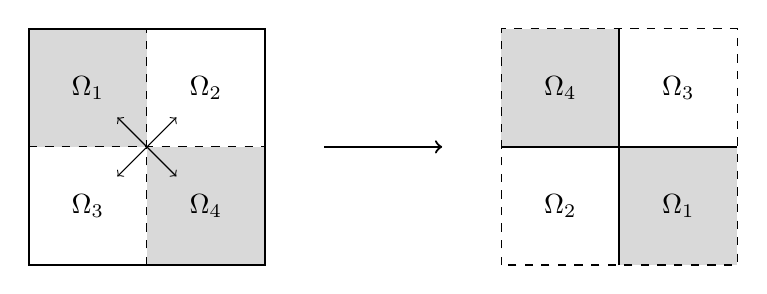
\begin{tikzpicture}[scale=1.5]
    % Original Grid
    \fill[gray!30] (0,1) rectangle (1, 2);
    \fill[gray!30] (1,0) rectangle (2, 1);
    \draw[<->] (0.75,0.75) -- (1.25,1.25);
    \draw[<->] (1.25,0.75) -- (0.75,1.25);
    \draw[thick] (0,0) rectangle (2,2);
    \draw[dashed] (1,0) -- (1,2);
    \draw[dashed] (0,1) -- (2,1);

    \node at (0.5,1.5) {$\Omega_1$};
    \node at (1.5,1.5) {$\Omega_2$};
    \node at (0.5,0.5) {$\Omega_3$};
    \node at (1.5,0.5) {$\Omega_4$};

    % Arrow
    \draw[->, thick] (2.5,1) -- (3.5,1);

    % Transformed Grid
    \begin{scope}[shift={(4,0)}]
        \fill[gray!30] (0,1) rectangle (1, 2);
        \fill[gray!30] (1,0) rectangle (2, 1);
        
        \draw[dashed] (0,0) rectangle (2,2);
        \draw[thick] (1,0) -- (1,2);
        \draw[thick] (0,1) -- (2,1);

        \node at (0.5,1.5) {$\Omega_4$};
        \node at (1.5,1.5) {$\Omega_3$};
        \node at (0.5,0.5) {$\Omega_2$};
        \node at (1.5,0.5) {$\Omega_1$};
    \end{scope}
\end{tikzpicture}
\end{frame}

\begin{frame}
\frametitle{Tobulo maišymo rezultatai}
\centering
\includegraphics[width=10cm]{paper/assets/optimal-mix-qnt-1.png}
\end{frame}

\begin{frame}
    \frametitle{Tobulo maišymo rezultatai}
    \centering
    \includegraphics[width=10cm]{paper/assets/mix-end-1.png}
\end{frame}

\begin{frame}
    \frametitle{Maišymas didesnėje erdvėje}
    \centering
    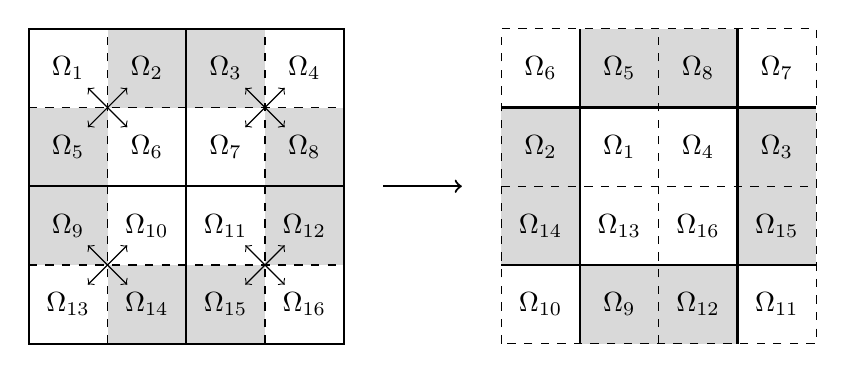
\begin{tikzpicture}
        % Original Grid
    
        \fill[gray!30] (1, 0) rectangle (3, 1);
        \fill[gray!30] (1, 3) rectangle (3, 4);
    
        \fill[gray!30] (0, 1) rectangle (1, 3);
        \fill[gray!30] (3, 1) rectangle (4, 3);
    
        \draw[thick] (0,0) rectangle (2,2);
        \draw[thick] (0,2) rectangle (2,4);
        \draw[thick] (2,0) rectangle (4,2);
        \draw[thick] (2,2) rectangle (4,4);
        \draw[dashed] (1,0) -- (1,4);
        \draw[dashed] (0,1) -- (4,1);
        \draw[dashed] (3,0) -- (3,4);
        \draw[dashed] (0,3) -- (4,3);
    
        \draw[<->] (0.75,0.75) -- (1.25,1.25);
        \draw[<->] (1.25,0.75) -- (0.75,1.25);
    
        \draw[<->] (2.75,0.75) -- (3.25,1.25);
        \draw[<->] (3.25,0.75) -- (2.75,1.25);
    
        \draw[<->] (0.75,2.75) -- (1.25,3.25);
        \draw[<->] (1.25,2.75) -- (0.75,3.25);
    
        \draw[<->] (2.75,2.75) -- (3.25,3.25);
        \draw[<->] (3.25,2.75) -- (2.75,3.25);
    
        \node at (0.5,3.5) {$\Omega_1$};
        \node at (1.5,3.5) {$\Omega_2$};
        \node at (0.5,2.5) {$\Omega_5$};
        \node at (1.5,2.5) {$\Omega_6$};
    
        \node at (2.5,3.5) {$\Omega_3$};
        \node at (3.5,3.5) {$\Omega_4$};
        \node at (2.5,2.5) {$\Omega_7$};
        \node at (3.5,2.5) {$\Omega_8$};
    
        \node at (0.5,1.5) {$\Omega_9$};
        \node at (1.5,1.5) {$\Omega_{10}$};
        \node at (0.5,0.5) {$\Omega_{13}$};
        \node at (1.5,0.5) {$\Omega_{14}$};
    
        \node at (2.5,1.5) {$\Omega_{11}$};
        \node at (3.5,1.5) {$\Omega_{12}$};
        \node at (2.5,0.5) {$\Omega_{15}$};
        \node at (3.5,0.5) {$\Omega_{16}$};
    
        % Arrow
        \draw[->, thick] (4.5,2) -- (5.5,2);
    
        % Transformed Grid
        \begin{scope}[shift={(6,0)}]
            \fill[gray!30] (1, 0) rectangle (3, 1);
            \fill[gray!30] (1, 3) rectangle (3, 4);
    
            \fill[gray!30] (0, 1) rectangle (1, 3);
            \fill[gray!30] (3, 1) rectangle (4, 3);
    
            \draw[dashed] (0,0) rectangle (4,4);
    
            \draw[dashed] (2,0) -- (2,4);
            \draw[dashed] (0,2) -- (4,2);
    
            \draw[thick] (1,0) -- (1,4);
            \draw[thick] (0,1) -- (4,1);
            \draw[thick] (3,0) -- (3,4);
            \draw[thick] (0,3) -- (4,3);
    
            \node at (0.5,3.5) {$\Omega_6$};
            \node at (1.5,3.5) {$\Omega_5$};
            \node at (0.5,2.5) {$\Omega_2$};
            \node at (1.5,2.5) {$\Omega_1$};
    
            \node at (2.5,3.5) {$\Omega_8$};
            \node at (3.5,3.5) {$\Omega_7$};
            \node at (2.5,2.5) {$\Omega_4$};
            \node at (3.5,2.5) {$\Omega_3$};
    
            \node at (0.5,1.5) {$\Omega_{14}$};
            \node at (1.5,1.5) {$\Omega_{13}$};
            \node at (0.5,0.5) {$\Omega_{10}$};
            \node at (1.5,0.5) {$\Omega_{9}$};
    
            \node at (2.5,1.5) {$\Omega_{16}$};
            \node at (3.5,1.5) {$\Omega_{15}$};
            \node at (2.5,0.5) {$\Omega_{12}$};
            \node at (3.5,0.5) {$\Omega_{11}$};
        \end{scope}
    \end{tikzpicture}
\end{frame}

\begin{frame}
    \frametitle{Maišymas didesnėje erdvėje}
    \centering
    \includegraphics[width=10cm]{paper/assets/mix-end-large-1.png}
\end{frame}

\begin{frame}
\frametitle{Išvados}
\begin{itemize}
    \item Atsitiktinio maišymo modelio rezultatai neatitinka realybėje pastebimų rezultatų, kai reakcija modeliuojama mažoje srityje, kurioje susiduria tik 4-ios mikrodalelės. Norint iš šio modelio išgauti tikrovę atitinkančius rezultatus yra būtina modeliuoti didesnę erdvės sritį.

    \item Tobulo išmaišymo modelio rezultatai atitinka realybėje pastebimą reakcijos pagreitėjimą.
    
    \item Modeliuojant didesnę erdvės sritį, tobulo išmaišymo modelio rezultatai kinta gana nežymiai, todėl maišymo modeliavimui užtenka modeliuoti mažą reakcijos erdvės sritį su 4-iom skirtingų medžiagų mikrodalelėmis

\end{itemize}
\end{frame}

\begin{frame}
\frametitle{Literatūros šaltiniai}
% \printbibliography
\end{frame}

\end{document}